% !TEX TS-program = xelatex
% !TEX encoding = UTF-8

% This is a simple template for a XeLaTeX document using the "article" class,
% with the fontspec package to easily select fonts.

\documentclass[11pt]{article} % use larger type; default would be 10pt

\usepackage{fontspec} % Font selection for XeLaTeX; see fontspec.pdf for documentation
\defaultfontfeatures{Mapping=tex-text} % to support TeX conventions like ``---''
\usepackage{xunicode} % Unicode support for LaTeX character names (accents, European chars, etc)
\usepackage{xltxtra} % Extra customizations for XeLaTeX
\usepackage{hyperref}
\usepackage{graphicx}

\hypersetup{
    colorlinks=true,
    linkcolor=blue,
    filecolor=magenta,      
    urlcolor=cyan,
}

\setmainfont{Charis SIL} % set the main body font (\textrm), assumes Charis SIL is installed
%\setsansfont{Deja Vu Sans}
%\setmonofont{Deja Vu Mono}

% other LaTeX packages.....
\usepackage{geometry} % See geometry.pdf to learn the layout options. There are lots.
\geometry{a4paper} % or letterpaper (US) or a5paper or....
%\usepackage[parfill]{parskip} % Activate to begin paragraphs with an empty line rather than an indent

\usepackage{graphicx} % support the \includegraphics command and options

\title{Synchronizační software pro potřeby live (a realtime) coding A/V praxe.}
\author{MgA. Kryštof Pešek}
\date{4. února 2017} % Activate to display a given date or no date (if empty),
         % otherwise the current date is printed 

\begin{document}
\maketitle

%\section*{Anotace:}

Charakter společných setkání, kterých jsem měl možnost se zůčastnit v rámci workshopu Martina Blažíčka, vychází z praxe takzvaného livecodingu, tj. produkování obrazu a zvuku v reálném čase za pomoci rozmanitých prostředí, které jsou k tomuto účelu vytvořeny.

Podobná praxe má, dnes především v zahraničí již dlouholetou tradici. Ačkoli se stále jedná o poměrně ojedinělou uměleckou praxi, komunity podobné těm mála domácím existují téměř již po celém světě. V Evropě nyní asi nejvíce ve Spojeném království nebo v Německu. Komunity se za posledních přibližně dvacet let přenesli z studentských a hudebních klubů nebo galerií do podoby reálných akademických programů a tato praxe je v různých podobách již i vyučována na prestižních uměleckých a technických univerzitách.

Od klasického pojetí práce v audiovizi, která dnes snad vychází nejvíce paradigmatu filmového průmyslu, tj. komponování audiovizuálního díla do uzamčeného tvaru určeného ke spotřebě, praxe livecodingu reflektuje nové technologické možnosti komputace obrazu i zvuku v reálném čase. Charakter audiovizuálního díla se tím poměrně dramaticky posouvá od uzamčeného komponovaného tvaru k více expresivní, živé produkci, která nutně obsahuje i prvky performativní. Tím vzniká naprosto paralelní větev k tradičně přijímané roli a představě o roli obrazu a zvuku. Samozřejmě spolu s novými možnostmi a specifickou kulturou vznikají i nové nároky na softwarová řešení, která v audiovizuální tvorbě tradičně (až na málo víjímek) stála spíše v pozici kompozičních prostředí směřující výsledek do výše zmíněného produktu, nežli nástrojů určených pro samotnou živou produkci.

Software, který je pro podobnou praxi vhodný, se vyznačuje zejména důrazem na možnost živé úpravy nástoje, který produkuje obraz nebo zvuk v reálném čase. Nástroje tak odpovídají spíše specifickým intuitivním nárokům, než soustředěné práci podobné metodě klacicky kompoziční. Hlavní požadavek stávajících i vznikajících programů a programovacích prostředí nejvíce požaduje možnosti zásahu do živě generované zvukového nebo obrazového výstupu ve vztahu na odehrávající se situaci či produkci ostatních spoluhráčů. Požadavky tak nově zahrnují spíše múzické požadavky na samotný software, které vychází dnes nejvíce z praxe než notně setrvačné teorie. V jednotlivých softwarových implementacích se tak jedná o jedinečné spojení technického, teoretického softwarově historického a naprosto praktického uvažování.

Vývoj samotného softwaru jde podle mého názor vždy ``ruku v ruce`` s konkrétními potřebami uživatelů/tvůrců softwaru a stěžejní je zde nutně možnost svobodné výměny informací, technická zdatnost a určitá míra skupinové shody (kompatibility) jednotlivých nástrojů a tvůrčích prostředí. Co je pak specifické na vývoji softwaru určeného pro popisovanou audiovizuáloní praxi je čistě fyzické a kulturní pojítko sdíleného času a prostředí ve kterém daný software vzniká. Tato spojitost nelze podcenit, protože představuje velmi výrazný rys; sdílené podmínky spojují i tak zásadně odlišná technologická prostředí, která by se za běžných okolností jen těžko takto konfrontovala.

Podobné mimořádné spojení probíhá na poměrně těžko dokumentovatelné bázi výskytu ``pokročilých hráčů`` na jednom místě v jeden čas. Jednotliví pokročilí uživatelé (hráči) tak tvoří mimořádnou vazbu, odehrávající se naprosto mimo racionální (softwarové) nebo systémové prostředí. To je způsobeno především tím, že potřeby každého hráče jsou velmi specifické a jednotná metodologie zde spíše neexistuje (nebo existovat nemůže).

\begin{center}
\begin{figure}
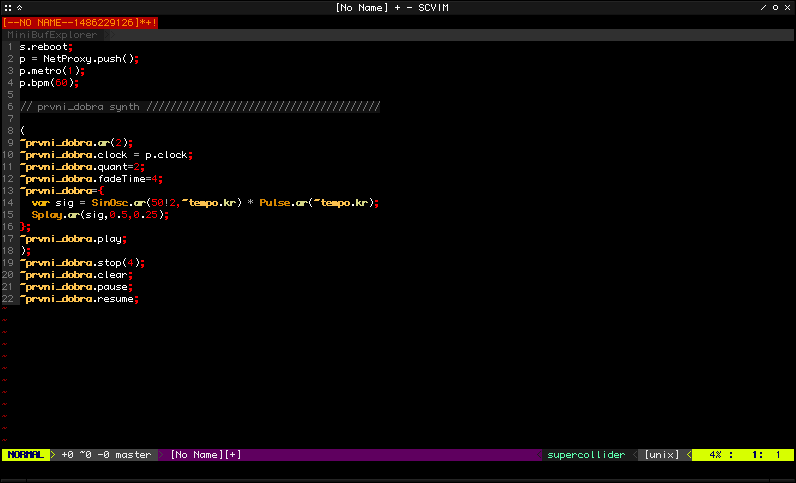
\includegraphics[width=1\textwidth]{screenshot.png}
\caption{ {\small příklad programovacího prostředí modifikovaného pro účely livecoding praxe, personalizovaný software nazvaný NetProxy v programovacím prostředí SuperCollider}}
\end{figure}
\end{center}


Software, který je k dispozici je často vyvíjen pro velmi specifické potřeby jednotlivých tvůrců a málokdy dochází na podobně volné (virtuózní) úrovni ke společné shodě. Vlastní vývoj vysoce personalizovaného softwaru pro podobné účely praxe je dnes velmi těžko monitorovatelný. Lze říci že v podobných komunitách se odhrává tolik vývoje jako je tvůrců. Stěžejní je zde fakt, že do komunitního rozvoje rodiny svobodných softwarových nástrojů, přispívají opravdu vrcholní tvůrci v oboru a uzavřenost je spíše okrajovým jevem. Podobný vývoj, nebo lépe řečeno vedení tvůrců k podrobnému popisu své praktické zkušenosti (a tím dokumentované personalizaci softwaru) je velmi přínosné ať už pro pro účely objevování konkrtétní jedinečné umělecké tvorby, nebo popisování kulturního hnutí jako takového.


Software, který vzniká dlouhodobě a vychází ze společných požadavků hráčů nese charatker synchronizačního modulu v programovacím prostředí SuperCollider. Software vyvýjený několika hráči, co možná nejméně zasahuje do uživatelských prostředí jednotlivých uživatelů. Řešení problému synchronizace vícero zvukových jednotek vychází z potřeb vzniklých při společné performatívní praxi.

Samotný vývoj synchronizačního softwaru, který je navržený pro synchronozaci v programovacím prostředí SuperCollider je vyvýjen omezeným počtem účastníků, ale je již poměrně snadno implementovatelný (a šiřitelný pod svobodnou licencí GNU/GPL 2.0). Software je k dispozici na webu a porálu komunitního softwaru GitHub.

Software zajišťuje synchronizaci zvukových serverů na několika simultárně běžících strojích přes síťový protokol UDP. Software \ je značně modulární a dovoluje vícero hráčům v prostředí SuperCollider sdílet  pomyslný  společný metronom, tím že dokáže distribuovat poměrně precizní časování (s odchylkou pod 10ms) značně přispívá k percepční kvalitě dané živé performance. 

Na vývoji softwaru se dále značnou měrou podílí Jáchym Pešek a na testování Alexandra Timpau a Martin Blažíček, příležitostně pak studenti Centra audiovizuálních studií a členové livecodingové skupiny Kolektiv.


%\subsection{}



\end{document}
